\documentclass{Note}
\usepackage{amsmath} %% for equation edit
\usepackage{amsfonts} %% for equation edit
\usepackage{ulem} %sout
\usepackage{amssymb}
\usepackage{graphicx}






\begin{document}
\title{Note:Lattice Bolzmann model for the simulation of the wave equation in curvilinear coordinates} 
%%% first author
\author{
     Email: jiaqi\_wang@sjtu.edu.cn
    } 

\maketitle

\section{cylinderical ducts}
\subsection{metric tensor and Christoffel symbols}
	For the duct case, cylinderical coordinates are given by the transformation


\begin{equation}
\begin{aligned}
x=rcos\theta\\
y=rsin\theta\\
z=z
\end{aligned}
\end{equation}

The metric tensor are derived:

\begin{equation}
\begin{aligned}
g_{rr}={\partial x\over \partial r}\cdot {\partial x\over \partial r}+{\partial y\over \partial r}\cdot {\partial y\over \partial r}+{\partial z\over \partial r}\cdot {\partial z\over \partial r}\\
={\partial rcos\theta\over \partial r}\cdot {\partial rcos\theta\over \partial r}+{\partial r sin\theta\over \partial r}\cdot {\partial r sin\theta\over \partial r}+{\partial z\over \partial r}\cdot {\partial z\over \partial r}\\
=cos^2\theta+sin^2\theta=1
\end{aligned}
\end{equation}

\begin{equation}
\begin{aligned}
g_{r\theta}=g_{\theta r}={\partial x\over \partial r}\cdot {\partial x\over \partial \theta}+{\partial y\over \partial r}\cdot {\partial y\over \partial \theta}+{\partial z\over \partial r}\cdot {\partial z\over \partial \theta}\\
={\partial rcos\theta\over \partial r}\cdot {\partial rcos\theta\over \partial \theta}+{\partial r sin\theta\over \partial r}\cdot {\partial r sin\theta\over \partial \theta}+{\partial z\over \partial r}\cdot {\partial z\over \partial \theta}\\
=-cos\theta\cdot r sin\theta+sin\theta\cdot r cos\theta +0=0
\end{aligned}
\end{equation}

\begin{equation}
\begin{aligned}
g_{r z}=g_{z r}={\partial x\over \partial r}\cdot {\partial x\over \partial z}+{\partial y\over \partial r}\cdot {\partial y\over \partial z}+{\partial z\over \partial r}\cdot {\partial z\over \partial z}\\
=0
\end{aligned}
\end{equation}

\begin{equation}
\begin{aligned}
g_{\theta \theta}={\partial x\over \partial \theta}\cdot {\partial x\over \partial \theta}+{\partial y\over \partial \theta}\cdot {\partial y\over \partial \theta}+{\partial z\over \partial \theta}\cdot {\partial z\over \partial \theta}\\
={\partial rcos\theta\over \partial \theta}\cdot {\partial rcos\theta\over \partial \theta}+{\partial r sin\theta\over \partial \theta}\cdot {\partial r sin\theta\over \partial \theta}+{\partial z\over \partial \theta}\cdot {\partial z\over \partial \theta}\\
=(-r sin\theta)^2+(r cos\theta)^2+0=r^2
\end{aligned}
\end{equation}

\begin{equation}
\begin{aligned}
g_{\theta z}=g_{z \theta}={\partial x\over \partial \theta}\cdot {\partial x\over \partial z}+{\partial y\over \partial \theta}\cdot {\partial y\over \partial z}+{\partial z\over \partial \theta}\cdot {\partial z\over \partial z}\\
=0
\end{aligned}
\end{equation}

\begin{equation}
\begin{aligned}
g_{z z}={\partial x\over \partial z}\cdot {\partial x\over \partial z}+{\partial y\over \partial z}\cdot {\partial y\over \partial z}+{\partial z\over \partial z}\cdot {\partial z\over \partial z}\\
=1
\end{aligned}
\end{equation}

Thus, we have:

\begin{equation}
\begin{aligned}
g_{ij}=
\begin{pmatrix}
1 & 0 & 0\\ 0 &r^2 & 0\\0 & 0 &1
\end{pmatrix}
\end{aligned}
\end{equation}

\begin{equation}
\begin{aligned}
g^{ij}=
\begin{pmatrix}
1 & 0 & 0\\ 0 &1/{r^2} & 0\\0 & 0 &1
\end{pmatrix}
\end{aligned}
\end{equation}

Next, we begin to derive the Christoffel symbols:
\begin{equation}
\begin{aligned}
\Gamma_{bc}^a=1/2 g^{ad}(g_{bd,c}+g_{cd,b}-g_{bc,d})
\end{aligned}
\end{equation}

ref:https://www.youtube.com/watch?v=Axhz7NAk4BM

1. for a=r, b=c=$\theta$, d can be r, $\theta$ , z, using Einstein summation convention:
\begin{equation}
\begin{aligned}
\Gamma_{\theta \theta}^r=1/2 g^{r d}(g_{\theta d,\theta}+g_{\theta d,\theta}-g_{\theta \theta,d})\\
=1/2 g^{r r}(g_{\theta r,\theta}+g_{\theta r,\theta}-g_{\theta \theta,r})+1/2 g^{r \theta}(g_{\theta \theta,\theta}+g_{\theta \theta,\theta}-g_{\theta \theta,\theta})+1/2 g^{r z}(g_{\theta z,\theta}+g_{\theta z,\theta}-g_{\theta \theta,z})\\
=1/2 g^{r r}({\partial g_{\theta r}\over\partial \theta}+{\partial g_{\theta r}\over\partial \theta}-{\partial g_{\theta \theta}\over\partial r})+1/2 g^{r \theta}({\partial g_{\theta \theta}\over\partial \theta}+{\partial g_{\theta \theta}\over\partial \theta}-{\partial g_{\theta \theta}\over\partial \theta})+1/2 g^{r z}({\partial g_{\theta z}\over\partial \theta}+{\partial g_{\theta z}\over\partial \theta}-{\partial g_{\theta \theta}\over\partial z})\\
=1/2\cdot (-2r)=-r
\end{aligned}
\end{equation}

2. for a=$\theta$, b=r, c=$\theta$, d can be r, $\theta$ , z, using Einstein summation convention:
\begin{equation}
\begin{aligned}
\Gamma_{r \theta}^\theta=1/2 g^{\theta d}(g_{r d,\theta}+g_{\theta d,r}-g_{r\theta,d})\\
=1/2 g^{\theta r}(g_{r r,\theta}+g_{\theta r,r}-g_{r \theta,r})+1/2 g^{\theta \theta}(g_{r \theta,\theta}+g_{\theta \theta,r}-g_{r \theta,\theta})+1/2 g^{\theta z}(g_{r z,\theta}+g_{\theta z,r}-g_{r \theta,z})\\
=1/2 g^{\theta r}({\partial g_{r r}\over\partial \theta}+{\partial g_{\theta r}\over\partial r}-{\partial g_{r \theta}\over\partial r})+1/2 g^{\theta \theta}({\partial g_{r \theta}\over\partial \theta}+{\partial g_{\theta \theta}\over\partial r}-{\partial g_{r \theta}\over\partial \theta})+1/2 g^{\theta z}({\partial g_{r z}\over\partial \theta}+{\partial g_{\theta z}\over\partial r}-{\partial g_{r \theta}\over\partial z})\\
=0+1/2\cdot (1/r^2)\cdot (2r)=1/r
\end{aligned}
\end{equation}

3.symmetry-> for a=$\theta$, b=$\theta$, c=r, d can be r, $\theta$ , z, using Einstein summation convention:
\begin{equation}
\begin{aligned}
\Gamma_{\theta r }^\theta=1/2 g^{ad}(g_{bd,c}+g_{cd,b}-g_{bc,d})=1/2 g^{ad}(g_{cd,b}+g_{bd,c}-g_{cb,d})\\=
\Gamma_{r \theta}^\theta=1/r
\end{aligned}
\end{equation}

4.for a=z, 
\begin{equation}
\begin{aligned}
\Gamma_{b c }^z=0
\end{aligned}
\end{equation}

5.for b=z, 
\begin{equation}
\begin{aligned}
\Gamma_{z c }^a=1/2 g^{ad}(g_{z d,c}+g_{cd,z}-g_{zc,d})=0
\end{aligned}
\end{equation}

6. for a=r, b=r,:
\begin{equation}
\begin{aligned}
\Gamma_{rc}^r=1/2 g^{rd}(g_{rd,c}+g_{cd,r}-g_{rc,d})=>(d=r)=>1/2 g^{rr}(g_{rr,c}+g_{cr,r}-g_{rc,r})=0
\end{aligned}
\end{equation}

7. for b=r, c=r,:
\begin{equation}
\begin{aligned}
\Gamma_{rr}^a=1/2 g^{ad}(g_{rd,r}+g_{rd,r}-g_{rr,d})=0
\end{aligned}
\end{equation}

Thus, we can conclude the 3D Christoffel symbols:
\begin{equation}
\begin{aligned}
\Gamma_{bc}^r=
\begin{pmatrix}
0 & 0 & 0\\ 0 &-r & 0\\0 & 0 &0
\end{pmatrix}
\end{aligned}
\end{equation}

\begin{equation}
\begin{aligned}
\Gamma_{bc}^\theta=
\begin{pmatrix}
0 & 1/r & 0\\1/r &0 & 0\\0 & 0 &0
\end{pmatrix}
\end{aligned}
\end{equation}

\begin{equation}
\begin{aligned}
\Gamma_{bc}^z=
\begin{pmatrix}
0 & 0 & 0\\ 0 &0 & 0\\0 & 0 &0
\end{pmatrix}
\end{aligned}
\end{equation}

\begin{figure}
  \centerline{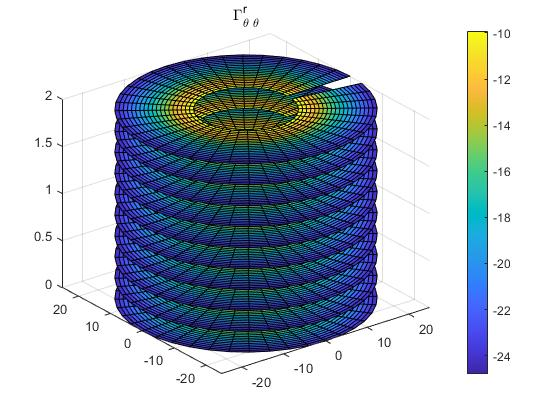
\includegraphics[width=4in]{Gamma_theta_theta^r.jpg}}
  \caption{$\Gamma_{\theta\theta}^r$}
  \end{figure}
  
\begin{figure}
  \centerline{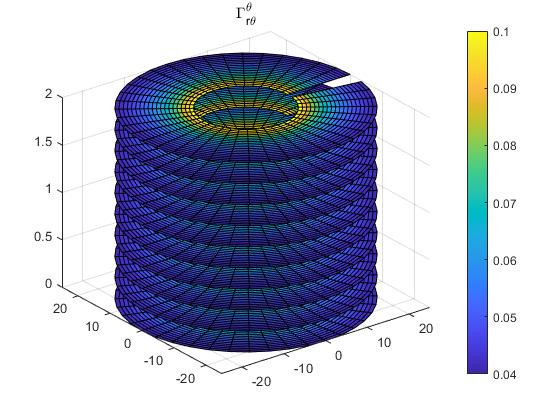
\includegraphics[width=4in]{Gamma_r_theta^theta.jpg}}
  \caption{$\Gamma_{r\theta}^\theta$}
  \end{figure}
  



\subsection{Intrinsic curvature}

ref:https://www.youtube.com/watch?v=YJFTWp31WhQ

The intrinstic curvature of a surface does not depend upon any embedding in higher dimensional space but depends upon relation between points within the surface.

A two dimensional being restricted to the surface of a sphere would draw a triagle whose angles sum to more than 180 degree and so would have to conclude that the surface is curved.

The Riemann tensor can tell if intrinsic curvature cccurs in a given space
\begin{equation}
\begin{aligned}
R_{\mu\gamma\beta}^\alpha={{\partial \Gamma_{\mu\beta}^\alpha}\over \partial x^\gamma}-{{\partial \Gamma_{\mu\gamma}^\alpha}\over \partial x^\beta}+\Gamma_{\mu\beta}^v \Gamma_{v\gamma}^\alpha-\Gamma_{\mu\gamma}^v\Gamma_{v\beta}^\alpha
\end{aligned}
\end{equation}

In 3-D the Riemann tensor has 81 components but with the following symmetry properties this number is reduced:

\begin{equation}
\begin{aligned}
R_{abcd}=R_{cdab}=-R_{bacd}=-R_{abdc}
\end{aligned}
\end{equation}


Due to these symmetries of the Riemann tensor the number of independent components is reduced to 6 independent components

\begin{equation}
\begin{aligned}
{n^2(n^2-1)\over 12}|_{n=3}=6 
\end{aligned}
\end{equation}

And the individual components are:
\begin{equation}
\begin{aligned}
R_{r\theta r}^\theta,R_{rzr}^{z},R_{\theta z \theta}^z, R_{r\theta r}^z, R_{\theta r \theta}^z, R_{zrz}^\theta
\end{aligned}
\end{equation}

In this cylinder case, all 81 of the Riemann tensor componets are zero in this space and all of the contraction of these components will also be zero because we are in flat Euclidean space.

The Ricci tensor is found by,
\begin{equation}
\begin{aligned}
R_{\mu v}=g^{\alpha\beta}R_{\alpha\mu\gamma\beta}
\end{aligned}
\end{equation}

The Ricci scalar is found using,
\begin{equation}
\begin{aligned}
R=g^{\mu v}R_{\mu v}
\end{aligned}
\end{equation}

So the Riemann tensor has identified this space as being curved since not all of its compoents are zero.

and the Ricci scalar or curvature scalar tells us that this space has constant curvature.

A sphere is a highly symmetric object, The Riemann tensor for a maximally symmteric space also be found using,
\begin{equation}
\begin{aligned}
R_{\rho \sigma \mu v}={R\over n(n-1)}(g_{\rho\mu}g_{\sigma v}-g_{\rho v}g_{\sigma\mu})
\end{aligned}
\end{equation}


\subsection{Cosmological constant}
The Einstein field equation,
\begin{equation}
\begin{aligned}
R_{\alpha v}-1/2g_{\alpha v}R={8\pi G\over c^4} T_{\alpha v}
\end{aligned}
\end{equation}















\end{document}


